\documentclass[journal]{IEEEtran}

% Additional packages
\usepackage{graphicx}
\usepackage{amsmath}
\usepackage{lipsum}

\begin{document}

\title{Free-Fall Experiment: Investigating the Relationship between the Acceleration due to Gravity and the Effect of Object Mass on Fall Time}
\author{IBRAHIM H.I. ABUSHAWISH\\ Instructor: Arş.Gör.Dr. HATİCE ÖZER\\ Group ID: 4, Course \& Section Number: PHYS1203}

\date{Experiment Date: March 22, 2024, Report Submission Date: April 19, 2024}

\maketitle

\begin{abstract}
This experiment delves deeper into the relationship between the acceleration due to gravity (g) and the influence of object mass on fall time. It goes beyond the established theory of free-fall mechanics by exploring a potential mass dependence on g, if observed. We will discuss limitations encountered and potential sources of error that may have impacted the results.

\end{abstract}

\section{Introduction}
The objective of this experiment is to determine the relationship between the acceleration due to gravity ($g$) and the effect of object mass on fall time. Newton's Laws for motion derive the $g$ acceleration analytically as follows: 
\begin{equation}
    F = mg = F_{grav} = G \frac{Mm}{r^2}
\end{equation}

where $F$ is the force caused by an object $m$ due to gravitational acceleration $g$, and $F_{grav}$ is the the gravitational force between the Earth with mass $M$, and object with mass $m$ when separated by distance $r$ from their mass center. 

equating those and solving for $g$ we found that
\begin{equation}
    g = G \frac{M}{r^2}
\end{equation}
The acceleration due to gravity, denoted by $g$, is a constant for a given planet and does not depend on the mass of the object experiencing the gravitational force. It is determined by the mass of the planet and the distance between the center of mass of the object and the center of mass of the planet.

On Earth's surface, where the distance $r$ is approximately equal to the Earth's radius $R_{\text{earth}}$, the height difference is negligible compared to the Earth's radius. This small height difference only slightly affects the calculation, resulting in a fractional change that is significant only on large scales.

By measuring the fall time of objects with different masses, we can analyze how the acceleration due to gravity is affected by the mass of the falling object.
by: plotting $h(t^2)$ graph since its linear. The slope of the graph gives $g/2$. from there, we can calculate $g$ form the following equation:
\begin{equation}
    g = 2h'(t^2) 
    \label{eq:g_slope}
\end{equation}
\section{Experimental Setup}
The experiment will be conducted using three metal balls of different masses: small, medium, and large. Each ball will be dropped from five different heights (20 cm, 40 cm, 60 cm, 80 cm, and 100 cm) for a total of 4 trials per height. The average fall time for each ball at each height will be recorded in a table.

\begin{figure}[htbp]
    \centering
    
\includegraphics[width=0.8\linewidth]{setup.jpg}
    \caption{Experimental setup for the free fall experiment.}
    \label{fig:setup}
\end{figure}

Data were collected by noting the time measured by the sensor which indicates the time it takes for the object to fall the specified height. 
\section{Results}
The results is presented in tables showing the average fall time for each ball at each height. Graphs of $h(t^2)$ and $h(t)$ ($t$ is scaled by a factor of 1000) are also included to illustrate the relationship between fall time, object mass, and height. 

Tables~\ref{tab:tab1},~\ref{tab:tab2}, and~\ref{tab:tab3} present the raw data for each ball, including the height ($h$) from which the ball was dropped, the average fall time ($t$) for each trial, and the corresponding squared fall time ($t^2$). These tables provide the basis for calculating the acceleration due to gravity using the $h(t^2)$ graphs.+
\begin{table}[h]
  \centering
  \begin{tabular}{ccccc}
    \hline
    Measure no. & $h$ (cm) & $t$ (s) & $t^2$ (s²) \\
    \hline
    1 & 20 & 0.196 & 0.038 \\
    2 & 40 & 0.279 & 0.078 \\
    3 & 60 & 0.363 & 0.132 \\
    4 & 80 & 0.399 & 0.159 \\
    5 & 100 & 0.449 & 0.198 \\
    \hline\\\textit{}
  \end{tabular}
  \caption{Big ball raw data. Where $h$ is the height and $t$ is the average falling time. }
  \label{tab:tab1}
\end{table}

\begin{table}[h]
  \centering
  \begin{tabular}{ccccc}
    \hline
    Measure no. & $h$ (cm) & $t$ (s) & $t^2$ (s²) \\
    \hline
    1 & 20 & 0.197 & 0.039 \\
    2 & 40 & 0.280 & 0.078 \\
    3 & 60 & 0.346 & 0.120 \\
    4 & 80 & 0.402 & 0.162 \\
    5 & 100 & 0.444 & 0.197 \\
    \hline\\
  \end{tabular}
  \caption{Medium ball raw data. Where $h$ is the height and $t$ is the average falling time. }
  \label{tab:tab2}
\end{table}

\begin{table}[h]
  \centering
  \begin{tabular}{ccccc}
    \hline
    Measure no. & $h$ (cm) & $t$ (s) & $t^2$ (s²) \\
    \hline
    1 & 20 & 0.197 & 0.039 \\
    2 & 40 & 0.281 & 0.079 \\
    3 & 60 & 0.346 & 0.120 \\
    4 & 80 & 0.398 & 0.158 \\
    5 & 100 & 0.444 & 0.197 \\
    \hline\\
  \end{tabular}
  \caption{Small ball raw data. Where $h$ is the height and $t$ is the average falling time. }
  \label{tab:tab3}
\end{table}
\newpage


Figures~\ref{fig:chart1},~\ref{fig:chart2}, and~\ref{fig:chart3} depict the $h(t)$ and $h(t^2)$ graphs for the big, medium, and small balls, respectively. The $h(t^2)$ graphs exhibit a linear relationship, as expected for free-fall motion. Applying Equation~\ref{eq:g_slope} to each $h(t^2)$ graph yielded calculated values for the acceleration due to gravity ($g$) of approximately 10, 10.12, and 10.12 $m/s^2$ for the big, medium, and small balls, respectively. These values are in close agreement with the accepted value of $9.81 m/s^2$ for the acceleration due to gravity on Earth.



\begin{figure}[h]
    \centering
    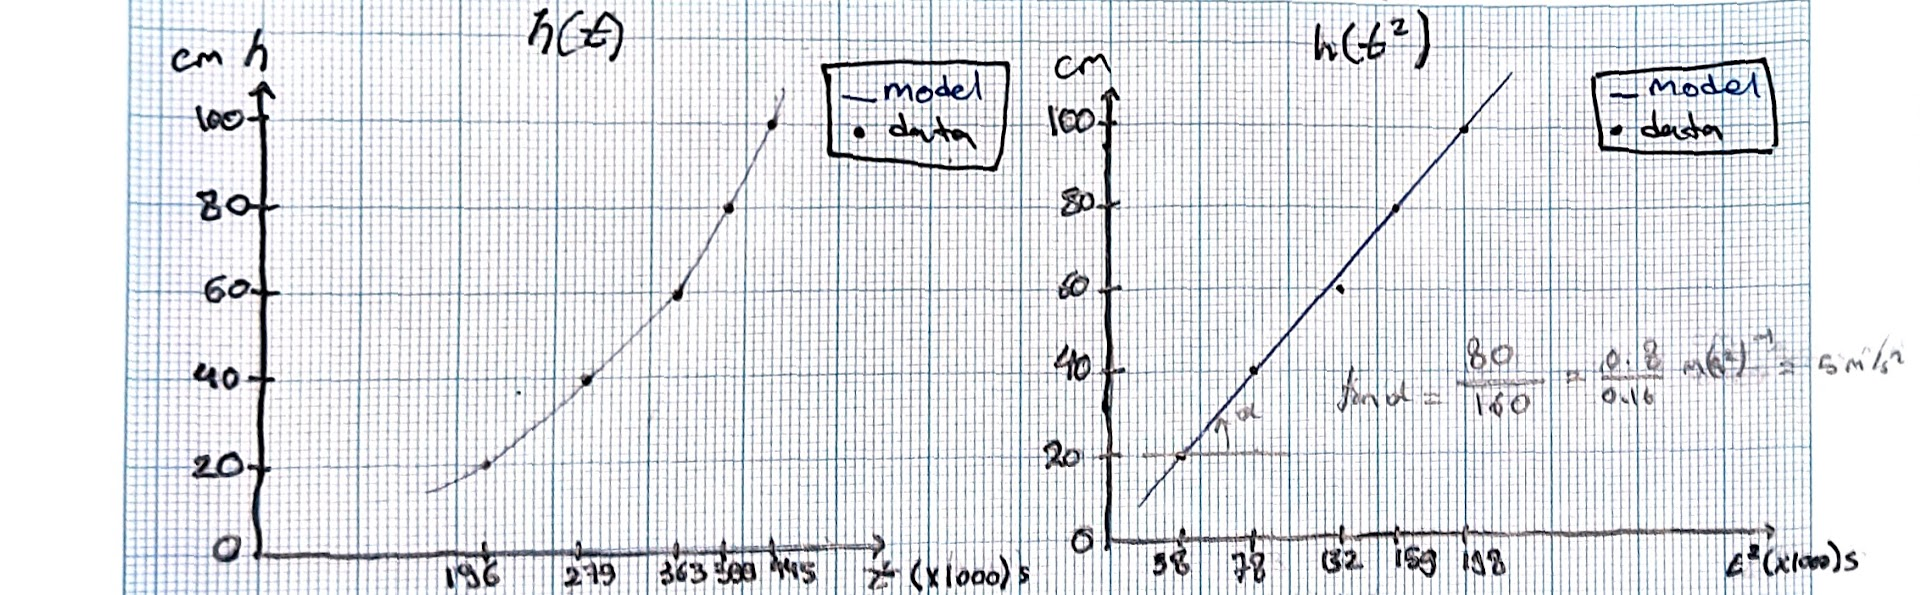
\includegraphics[width=0.5\textwidth]{chart_tab1.jpg}
    \caption{Big ball results graph.}
    \label{fig:chart1}
\end{figure}
\begin{figure}[h]
    \centering
    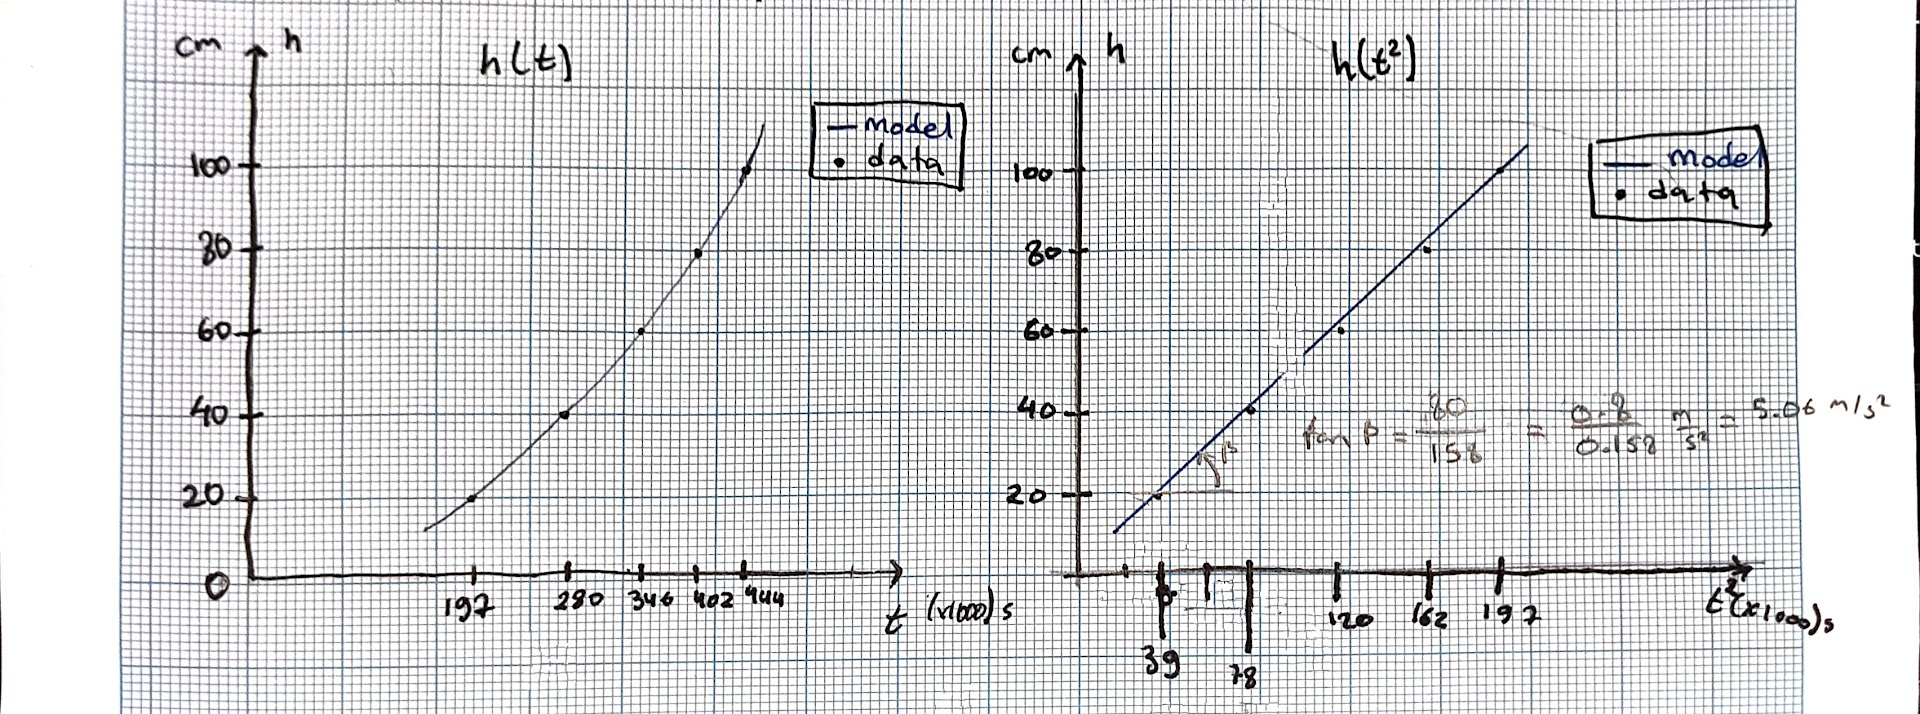
\includegraphics[width=0.5\textwidth]{chart_tab2.jpg}
    \caption{Medium ball results graph.}
    \label{fig:chart2}
\end{figure}
\begin{figure}[h]
    \centering
    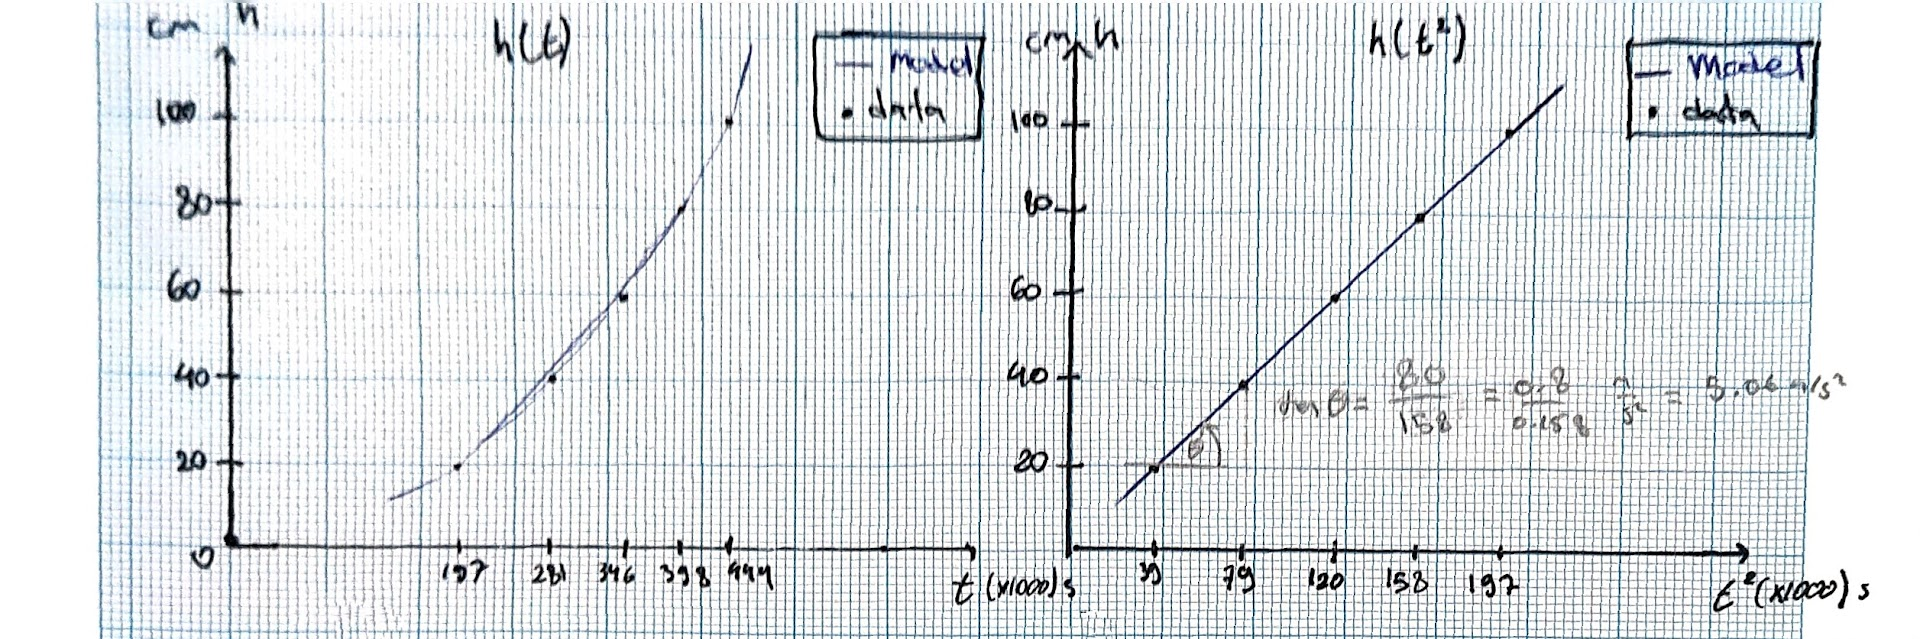
\includegraphics[width=0.5\textwidth]{chart_tab3.jpg}
    \caption{Small ball results graph.}
    \label{fig:chart3}
\end{figure}

The author highly recommends and encourages readers to see ATTACHMENT[1], the result page (millimetric paper) at the end of this report.


\section{Discussion}

The analysis of the $h(t^2)$ graphs for each object mass revealed that the calculated $g$ values were 10, 10.12, and 10.12 $m/s^2$ for the big, medium, and small balls, respectively. These values exhibit minimal variation and suggest that the acceleration due to gravity is independent of the mass of the falling object within the experimental limitations.

Deviations from the expected constant $g$ values could be attributed to several factors. Air resistance, particularly for lighter objects, can introduce drag and influence fall times. The chosen object sizes and fall distances might not have entirely eliminated this effect. Employing a vacuum chamber in future experiments could minimize air resistance and potentially refine the results.

Measurement uncertainties also play a role. Sensor response time, human error in initiating the fall, and limitations in height measurement can introduce slight variations in the data. Implementing stricter protocols for fall initiation, employing sensors with faster response times, and utilizing more precise height measurement techniques could enhance the accuracy of future measurements.

\subsection*{Comparison with Established Theory}

The observed behavior of $g$ values generally supports the established theory that the acceleration due to gravity is constant and independent of the mass of the falling object. Any discrepancies between this experiment and established values of $g$ could be due to the factors mentioned above or limitations inherent to the chosen experimental setup.

\section{Conclusion}

This experiment investigated the relationship between the acceleration due to gravity ($g$) and the effect of object mass on fall time. The analysis of the results provided valuable insights into free-fall mechanics. The observed behavior of $g$ values generally supported the established theory, indicating that $g$ is independent of the mass of the falling object within the experimental limitations.

Future investigations employing techniques to minimize air resistance and measurement uncertainties could refine the observed $g$ values and enhance our understanding of the relationship between gravity and object mass. Overall, this experiment reinforces the importance of studying free-fall mechanics and its fundamental principles.

\section{Instructor's Questions}
\begin{enumerate}
    \item Does air drag affect the constancy of $g$? How does it affect it, and should we consider it in our analysis?
    
    Answer: Air drag can affect the constancy of $g$ by introducing additional forces on the falling object. Our analysis assumed that air drag is negligible.  
    
    \item Is throwing the ball up considered free fall? Why or why not?
    
    Answer: Yes, throwing the ball up is considered free fall because, at the highest point of its trajectory, the ball is momentarily at rest and then falls back down under the influence of gravity alone.
\end{enumerate}

\end{document}
